\documentclass[10pt]{beamer}
\usepackage{../../shared/styles/custom}
\usepackage{../../shared/styles/conventions}

% Remove navigation symbols
\setbeamertemplate{navigation symbols}{}

% Add fitpic for image fitting
\newcommand{\fitpic}[1]{\begin{adjustbox}{max width=\linewidth, max totalheight=0.78\textheight}#1\end{adjustbox}}

\graphicspath{ {../assets/bias-variance/figures/} }

\title{The Bias-Variance Tradeoff: A Deep Dive}
\date{\today}
\author{Nipun Batra and teaching staff}
\institute{IIT Gandhinagar}
\begin{document}
\maketitle

\begin{frame}{Table of Contents}
\tableofcontents
\end{frame}

\section{Understanding the Problem Setup}

\begin{frame}{The Learning Problem: A Real-World Example}
\begin{definitionbox}{Our Scenario}
\textbf{Goal:} Predict housing prices based on house area
\end{definitionbox}

\begin{examplebox}{The True Relationship}
\textbf{Unknown to us:} There exists a true function $f_{\theta_{\text{true}}}$ that perfectly relates area to price:
$$y_t = f_{\theta_{\text{true}}}(x_t)$$
\end{examplebox}

\begin{center}
\fitpic{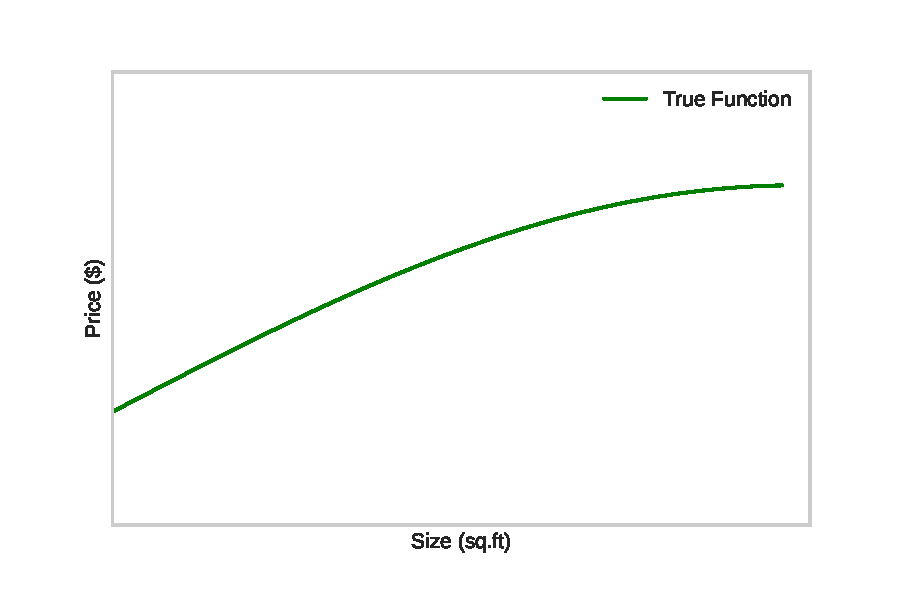
\includegraphics[width=0.7\textwidth]{../assets/bias-variance/figures/true.pdf}}
\end{center}

\begin{keypointsbox}
\textbf{Key Challenge:} We never know $f_{\theta_{\text{true}}}$ - we must estimate it from data!
\end{keypointsbox}
\end{frame}

\begin{frame}{The Three Sources of Prediction Error}
\begin{alertbox}{Fundamental Question}
\textbf{Why do our predictions fail?} What causes the difference between our predictions and reality?
\end{alertbox}

\begin{definitionbox}{Three Universal Sources of Error}
\textbf{Every machine learning prediction suffers from:}
\begin{enumerate}
\item \textbf{Noise} - Irreducible randomness in the data
\item \textbf{Bias} - Systematic errors from model assumptions
\item \textbf{Variance} - Sensitivity to particular training sets
\end{enumerate}
\end{definitionbox}

\begin{keypointsbox}
\textbf{The Tradeoff:} We can often reduce bias OR variance, but not both simultaneously!
\end{keypointsbox}

\begin{examplebox}{Preview}
\textbf{Coming up:} We'll see exactly how these three components combine mathematically and how to balance them.
\end{examplebox}
\end{frame}

\section{Source 1: Noise - The Irreducible Error}

\begin{frame}{Understanding Noise: The Fundamental Limitation}
\begin{definitionbox}{What is Noise?}
\textbf{Noise} represents factors affecting the target that we cannot observe or control
\end{definitionbox}

\begin{examplebox}{Real-World Noise Sources}
\textbf{In housing prices:}
\begin{itemize}
\item House condition (hard to measure precisely)
\item Neighborhood market dynamics
\item Buyer's personal preferences
\end{itemize}
\end{examplebox}
\end{frame}

\begin{frame}{Noise: Why It's Irreducible}
\begin{examplebox}{More Noise Sources}
\textbf{Additional factors we cannot control:}
\begin{itemize}
\item Economic conditions on sale day
\item Unmeasurable aesthetic factors
\item Random market fluctuations
\item Measurement errors in data collection
\end{itemize}
\end{examplebox}

\begin{alertbox}{Key Insight}
\textbf{Irreducible Error:} No matter how sophisticated our model, noise cannot be eliminated!
\end{alertbox}
\end{frame}

\begin{frame}{Noise: Mathematical Formulation}
\begin{keypointsbox}{The Noisy Relationship}
\textbf{True relationship becomes:}
$$y_t = f_{\theta_{\text{true}}}(x_t) + \epsilon_t$$
where $\epsilon_t \sim \mathcal{N}(0, \sigma^2)$ is the noise term
\end{keypointsbox}

\begin{center}
\fitpic{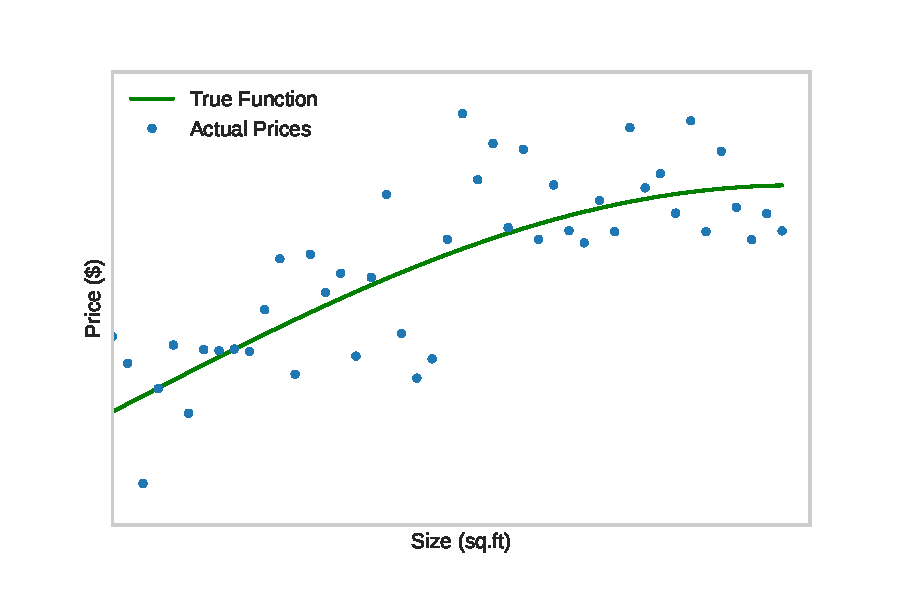
\includegraphics[width=0.7\textwidth]{../assets/bias-variance/figures/data.pdf}}
\end{center}
\end{frame}

\begin{frame}{Noise: Mathematical Properties}
\begin{definitionbox}{Key Properties of Noise}
\begin{itemize}
\item \textbf{Zero mean:} $E[\epsilon_t] = 0$ (unbiased)
\item \textbf{Constant variance:} $\text{Var}(\epsilon_t) = \sigma^2$
\item \textbf{Independent:} Each observation's noise is independent
\end{itemize}
\end{definitionbox}

\begin{keypointsbox}{Why These Properties Matter}
\begin{itemize}
\item \textbf{Zero mean:} Noise doesn't systematically bias our target
\item \textbf{Constant variance:} Prediction uncertainty is consistent
\item \textbf{Independence:} One data point's noise doesn't affect others
\end{itemize}
\end{keypointsbox}
\end{frame}

\begin{frame}{Visualizing Noise: Data Distribution}
\begin{center}
\fitpic{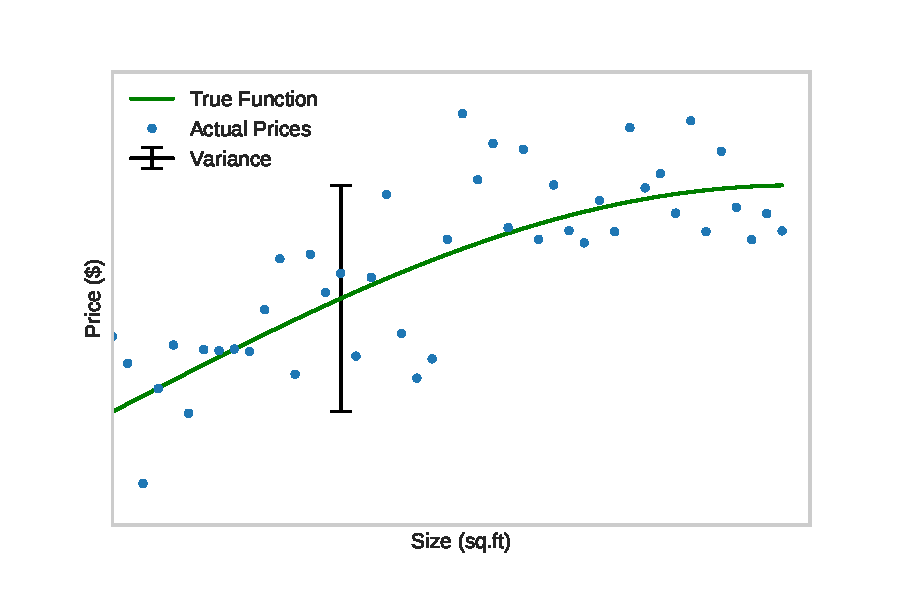
\includegraphics[width=0.8\textwidth]{../assets/bias-variance/figures/data_var.pdf}}
\end{center}

\begin{keypointsbox}
\textbf{Key Observation:} 
\begin{itemize}
\item Data points scatter around the true function
\item The spread (variance) is constant: $\sigma^2$
\item This randomness cannot be removed by better modeling
\end{itemize}
\end{keypointsbox}

\begin{alertbox}{Implication for ML}
\textbf{Lower bound on error:} Any model will have at least $\sigma^2$ error due to noise
\end{alertbox}
\end{frame}

\section{Source 2: Bias - Systematic Model Limitations}

\begin{frame}{Understanding Bias: Model Flexibility}
\begin{definitionbox}{What is Bias?}
\textbf{Bias} measures how well our model class can represent the true function
\end{definitionbox}

\begin{examplebox}{Extreme Example: Constant Function}
\textbf{Model choice:} $\hat{f}(x) = c$ (constant, regardless of house size)

\textbf{Question:} Can this model capture the true price-size relationship?
\end{examplebox}
\end{frame}

\begin{frame}{Bias: Visualizing the Problem}
\begin{center}
\fitpic{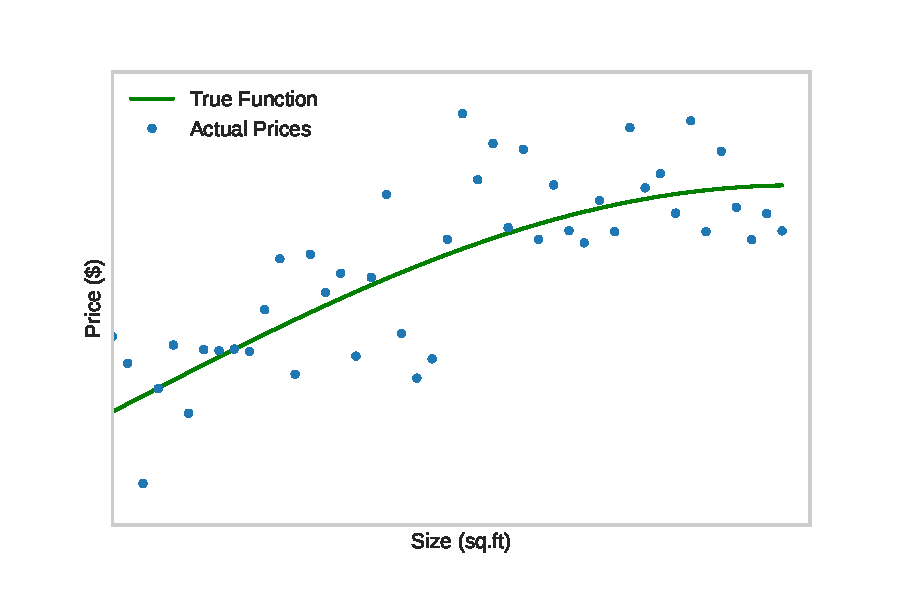
\includegraphics[width=0.8\textwidth]{../assets/bias-variance/figures/biasn_1.pdf}}
\end{center}

\begin{alertbox}
\textbf{Obvious Problem:} A constant function cannot capture any relationship with house size!
\end{alertbox}
\end{frame}

\begin{frame}{Bias: Fitting a Constant Model}
\begin{center}
\fitpic{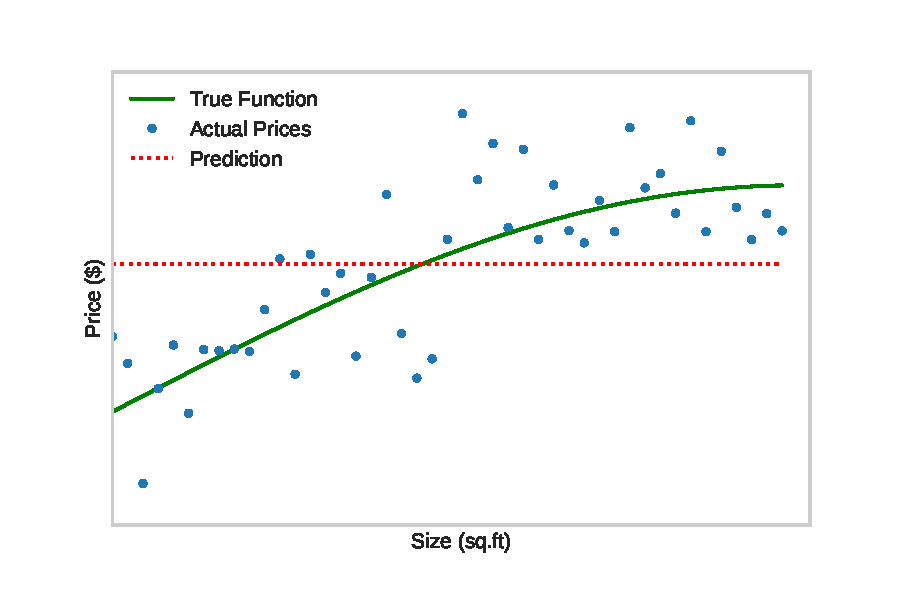
\includegraphics[width=0.8\textwidth]{../assets/bias-variance/figures/biasn_2.pdf}}
\end{center}

\begin{keypointsbox}
\textbf{Best Constant Fit:} 
\begin{itemize}
\item The optimal constant is the average of all prices
\item But this completely ignores the size information!
\item Large systematic errors remain
\end{itemize}
\end{keypointsbox}
\end{frame}

\begin{frame}{Bias: Visualizing the Systematic Error}
\begin{center}
\fitpic{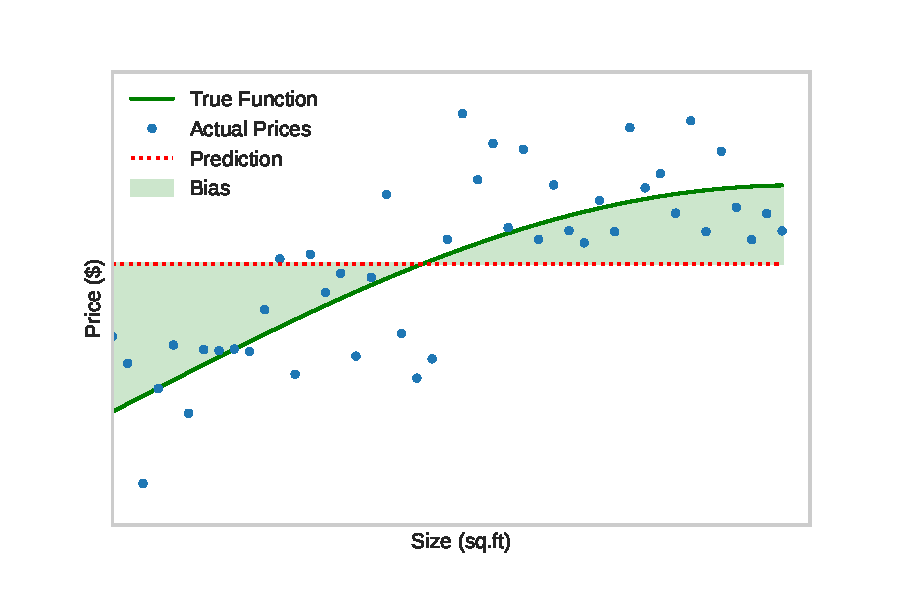
\includegraphics[width=0.8\textwidth]{../assets/bias-variance/figures/biasn_3.pdf}}
\end{center}

\begin{definitionbox}{Bias Definition}
$$\text{Bias}(x) = f_{\theta_{\text{true}}}(x) - E[\hat{f}(x)]$$
\textbf{The systematic difference between truth and average prediction}
\end{definitionbox}

\begin{alertbox}{Key Insight}
\textbf{High bias = Underfitting:} Model assumptions are too restrictive
\end{alertbox}
\end{frame}

\begin{frame}{Multiple Datasets: Understanding Variability}
\begin{keypointsbox}
\textbf{Crucial Insight:} Many different datasets are possible from the same true relationship!
\end{keypointsbox}

\begin{center}
\fitpic{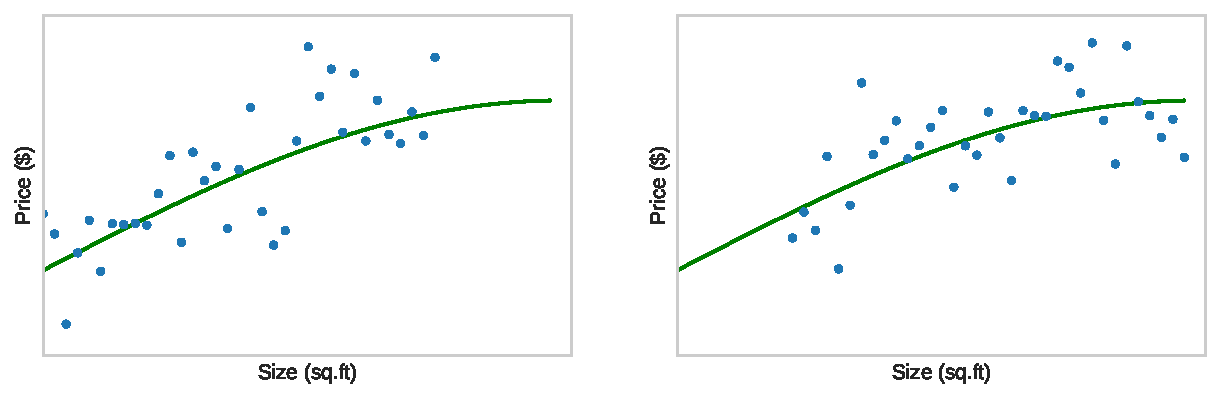
\includegraphics[width=0.95\textwidth]{../assets/bias-variance/figures/bias1.pdf}}
\end{center}

\begin{examplebox}
\textbf{Same underlying relationship, different data points due to:}
\begin{itemize}
\item Random sampling of houses
\item Different noise realizations
\item Natural variation in the population
\end{itemize}
\end{examplebox}
\end{frame}

\begin{frame}{Fitting Models to Different Datasets}
\begin{center}
\fitpic{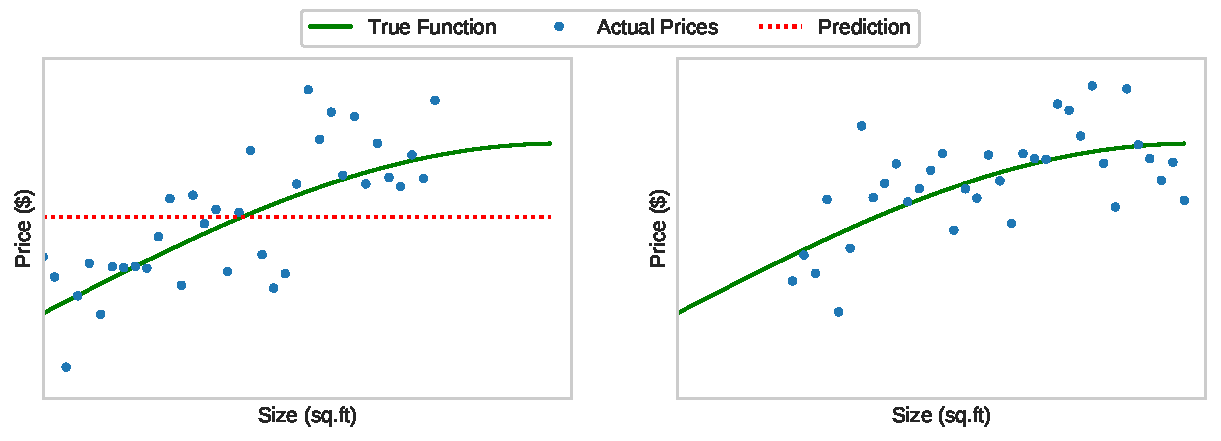
\includegraphics[width=0.95\textwidth]{../assets/bias-variance/figures/bias2.pdf}}
\end{center}

\begin{keypointsbox}
\textbf{Question:} If we fit the same model type (constant) to different datasets, what happens?
\end{keypointsbox}
\end{frame}

\begin{frame}{Different Predictions from Different Datasets}
\begin{center}
\fitpic{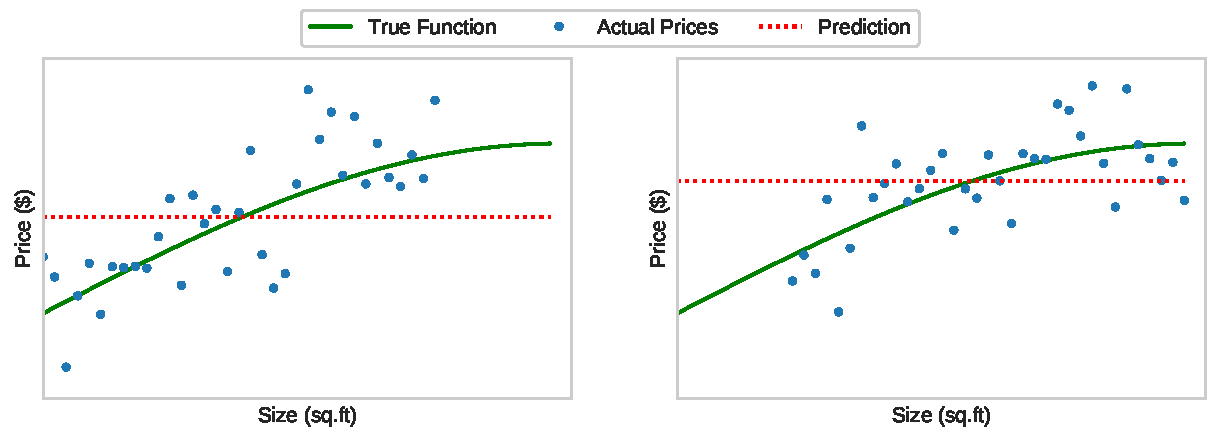
\includegraphics[width=0.95\textwidth]{../assets/bias-variance/figures/bias3.pdf}}
\end{center}

\begin{alertbox}
\textbf{Key Observation:} Even with the same model type, we get different predictions!
\end{alertbox}

\begin{definitionbox}
\textbf{This variability leads us to two concepts:}
\begin{itemize}
\item \textbf{Average prediction:} What happens "on average" across all possible datasets
\item \textbf{Prediction variance:} How much predictions vary across datasets
\end{itemize}
\end{definitionbox}
\end{frame}

\begin{frame}{Many Datasets: The Full Picture}
\begin{center}
\fitpic{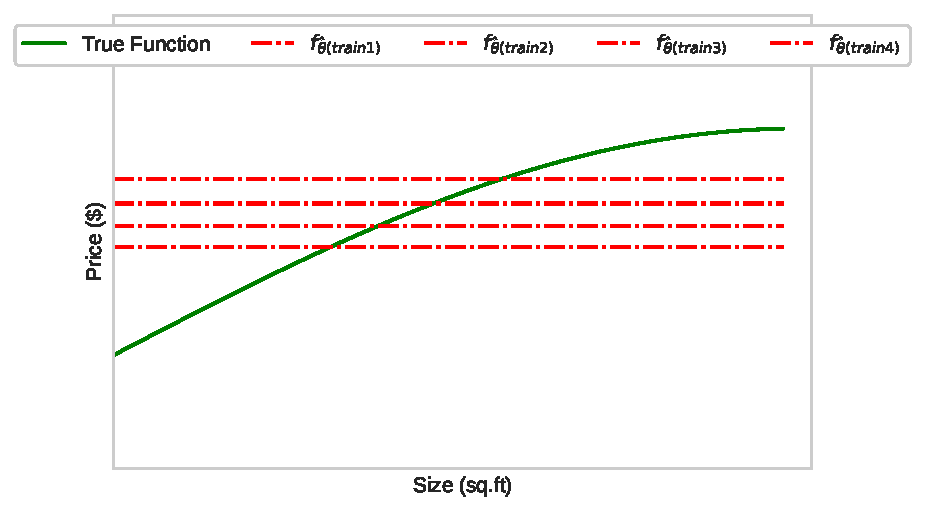
\includegraphics[width=0.8\textwidth]{../assets/bias-variance/figures/bias4.pdf}}
\end{center}

\begin{keypointsbox}
\textbf{Multiple Datasets:} Each gives a slightly different constant fit
\end{keypointsbox}

\begin{examplebox}
\textbf{The Big Question:} What is the "typical" or "expected" prediction our model makes?
\end{examplebox}
\end{frame}

\begin{frame}{The Average Model: Expected Prediction}
\begin{center}
\fitpic{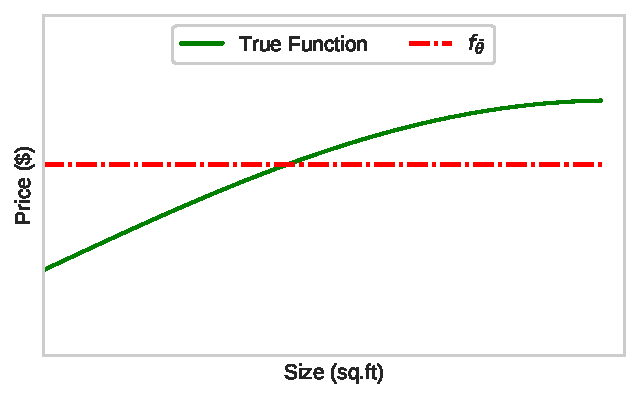
\includegraphics[width=0.7\textwidth]{../assets/bias-variance/figures/bias5.pdf}}
\end{center}

\begin{definitionbox}{Expected Prediction}
$$E[\hat{f}(x)] = \text{Average prediction across all possible training sets}$$
\end{definitionbox}

\begin{keypointsbox}
\textbf{For constant models:} The expected prediction is the expected value of the target variable
\end{keypointsbox}
\end{frame}

\begin{frame}{Bias: The Final Definition}
\begin{definitionbox}{Bias Formula}
$$\text{Bias}(x) = f_{\theta_{\text{true}}}(x) - E[\hat{f}(x)]$$
\textbf{Difference between truth and expected prediction}
\end{definitionbox}

\begin{center}
\fitpic{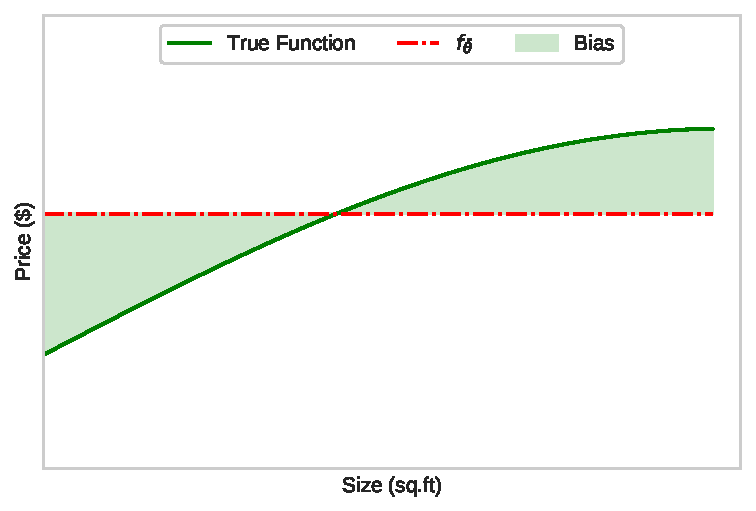
\includegraphics[width=0.7\textwidth]{../assets/bias-variance/figures/bias6.pdf}}
\end{center}

\begin{keypointsbox}
\textbf{Interpretation:}
\begin{itemize}
\item \textbf{Large bias:} Model class cannot represent truth well
\item \textbf{Small bias:} Model class is flexible enough
\item \textbf{Bias measures systematic error, not random error}
\end{itemize}
\end{keypointsbox}
\end{frame}

\begin{frame}{Model Complexity vs Bias: The Relationship}
\begin{keypointsbox}
\textbf{Universal Pattern:}
\begin{itemize}
\item \textbf{Increase complexity} → Model becomes more flexible
\item \textbf{More flexible} → Can better approximate true function
\item \textbf{Better approximation} → \textcolor{blue}{Bias decreases}
\end{itemize}
\end{keypointsbox}

\begin{center}
\fitpic{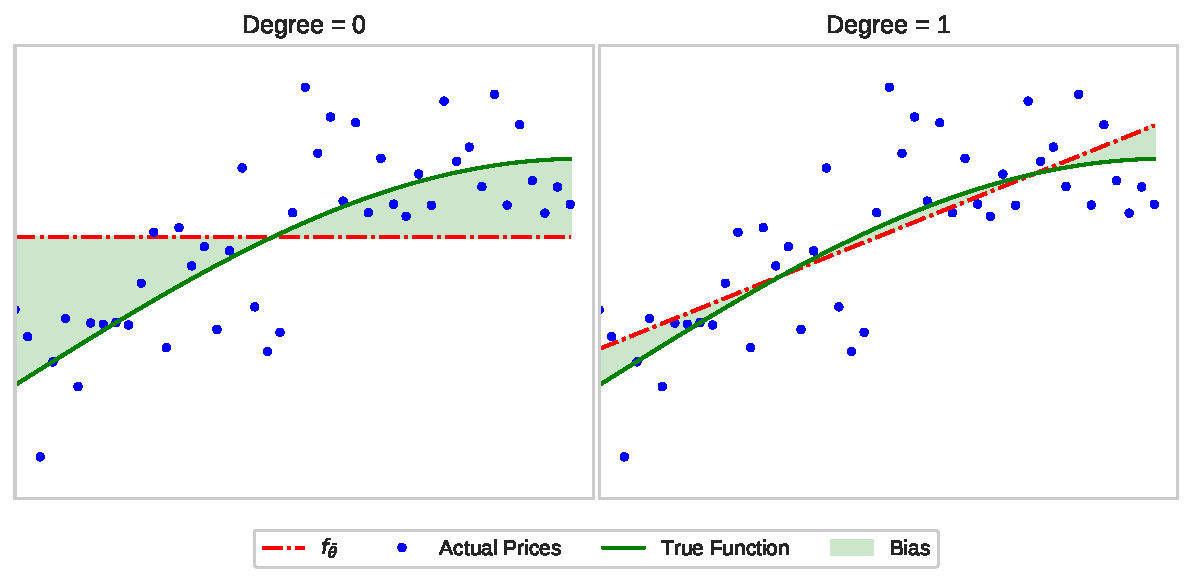
\includegraphics[width=0.95\textwidth]{../assets/bias-variance/figures/bias7.pdf}}
\end{center}

\begin{examplebox}
\textbf{Progression:} Constant → Linear → Quadratic → Cubic ...
\end{examplebox}
\end{frame}

\begin{frame}{High-Complexity Models: Near-Zero Bias}
\begin{center}
\fitpic{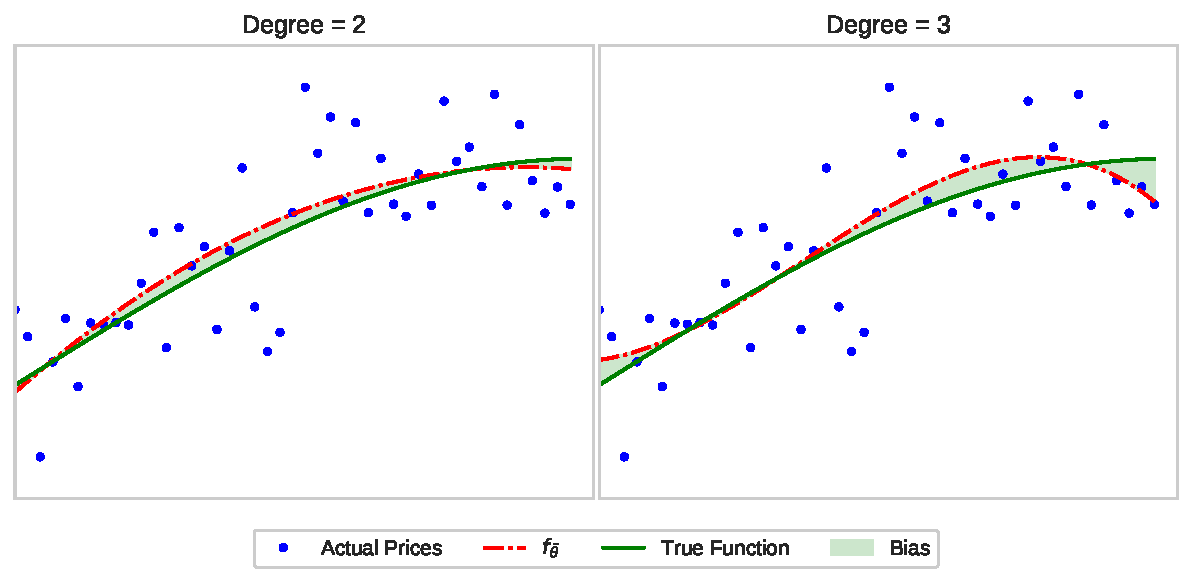
\includegraphics[width=0.95\textwidth]{../assets/bias-variance/figures/bias8.pdf}}
\end{center}

\begin{alertbox}
\textbf{High-Degree Polynomials:} Can approximate almost any smooth function!
\end{alertbox}

\begin{definitionbox}
\textbf{Bias-Complexity Relationship:}
\begin{itemize}
\item \textbf{Low complexity:} High bias (underfitting)
\item \textbf{High complexity:} Low bias (but...)
\end{itemize}
\end{definitionbox}

\begin{keypointsbox}
\textbf{The "But":} Low bias comes at a cost - we'll see what next!
\end{keypointsbox}
\end{frame}

\section{Source 3: Variance - Dataset Sensitivity}

\begin{frame}{From Bias to Variance: The Other Side}
\begin{alertbox}
\textbf{We've seen:} High-complexity models have low bias

\textbf{Question:} If low bias is good, why not always use high-complexity models?
\end{alertbox}

\begin{definitionbox}{Enter Variance}
\textbf{Variance} measures how much predictions change when we train on different datasets
\end{definitionbox}

\begin{keypointsbox}
\textbf{Intuition:} 
\begin{itemize}
\item Simple models: Stable, consistent predictions
\item Complex models: Highly sensitive to specific training data
\end{itemize}
\end{keypointsbox}

\begin{examplebox}{Coming Up}
\textbf{We'll see:} As complexity increases, variance increases dramatically!
\end{examplebox}
\end{frame}

\begin{frame}{Understanding Variance: Prediction Consistency}
\begin{definitionbox}{Variance Definition}
\textbf{Variance} = How much do predictions vary across different training sets?
$$\text{Var}(\hat{f}(x)) = E[(\hat{f}(x) - E[\hat{f}(x)])^2]$$
\end{definitionbox}

\begin{center}
\fitpic{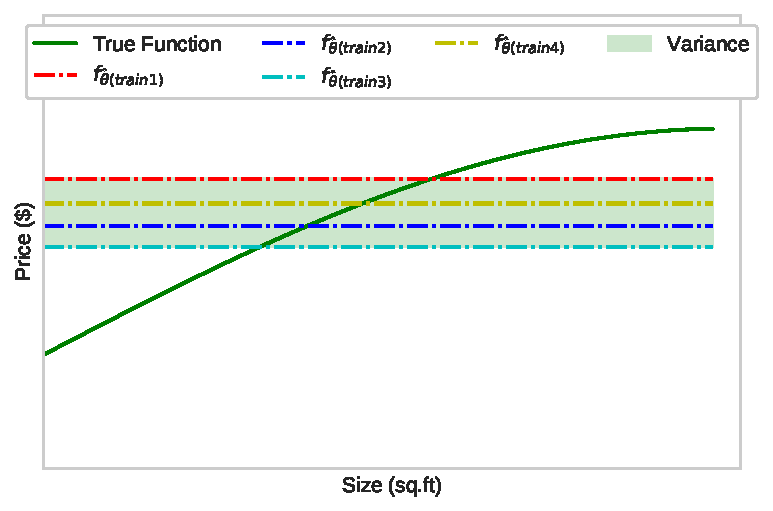
\includegraphics[width=0.7\textwidth]{../assets/bias-variance/figures/var1.pdf}}
\end{center}

\begin{keypointsbox}
\textbf{Key Concept:} Variance measures prediction instability
\begin{itemize}
\item \textbf{Low variance:} Consistent predictions across datasets
\item \textbf{High variance:} Wildly different predictions across datasets
\end{itemize}
\end{keypointsbox}
\end{frame}

\begin{frame}{Low Complexity: Low Variance}
\begin{keypointsbox}
\textbf{Simple Models (e.g., linear):}
\begin{itemize}
\item Few parameters to estimate
\item Robust to data variations
\item Consistent predictions
\end{itemize}
\end{keypointsbox}

\begin{center}
\fitpic{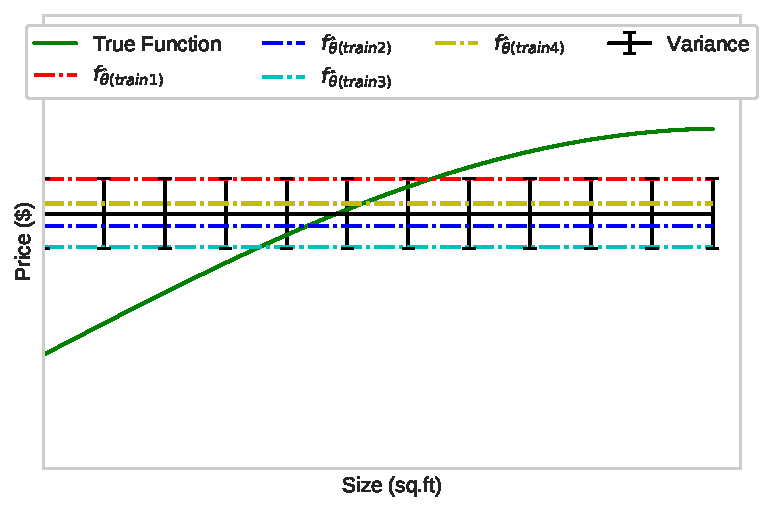
\includegraphics[width=0.7\textwidth]{../assets/bias-variance/figures/var2.pdf}}
\end{center}

\begin{definitionbox}
\textbf{Low Variance = Stability:} Predictions don't change much with different training sets
\end{definitionbox}
\end{frame}

\begin{frame}{High Complexity: The Variance Problem Emerges}
\begin{center}
\fitpic{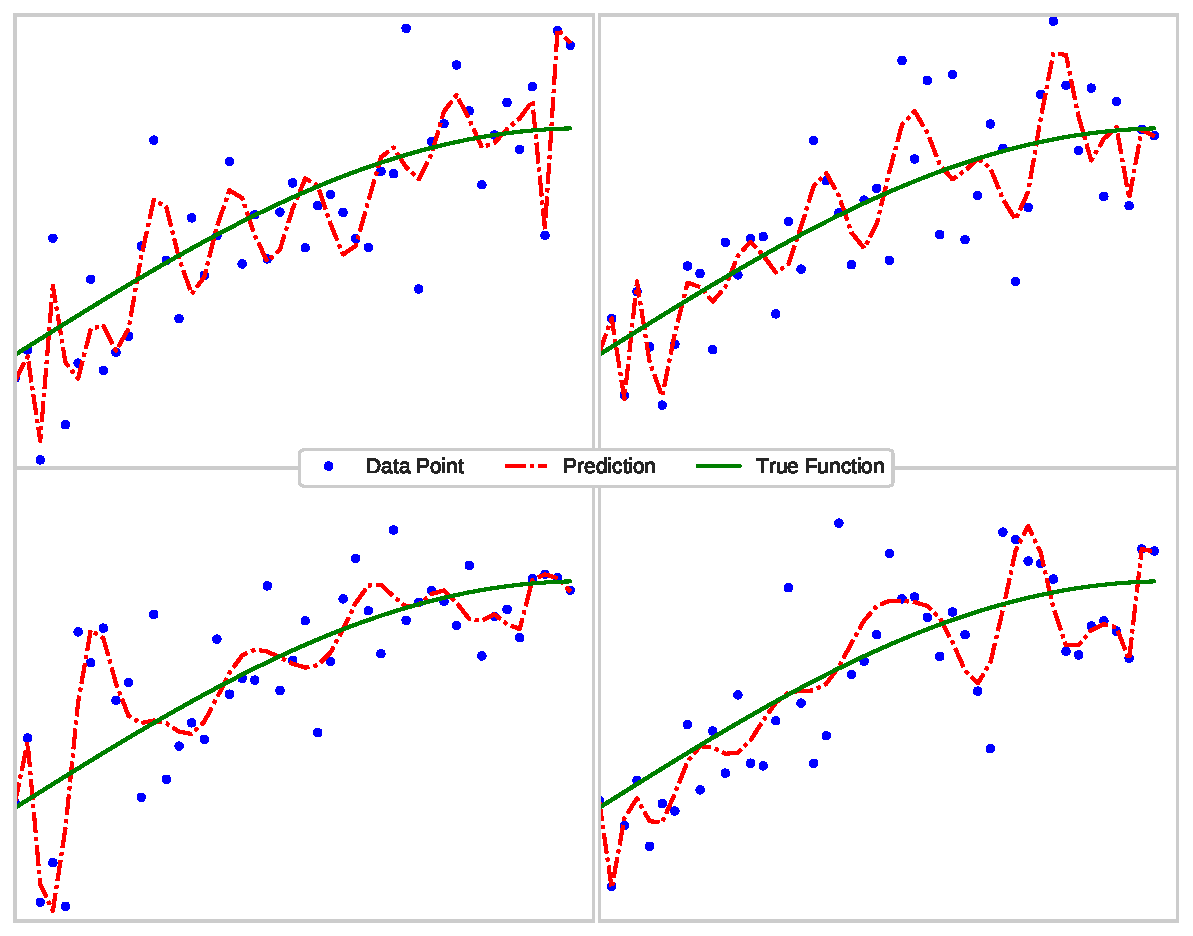
\includegraphics[width=0.7\textwidth]{../assets/bias-variance/figures/var3.pdf}}
\end{center}

\begin{alertbox}
\textbf{Warning Signs:} 
\begin{itemize}
\item Models look very different across datasets
\item Predictions becoming unreliable
\item High sensitivity to specific data points
\end{itemize}
\end{alertbox}
\end{frame}

\begin{frame}{High Complexity: Extreme Variance}
\begin{keypointsbox}
\textbf{Complex Models (e.g., high-degree polynomials):}
\begin{itemize}
\item Many parameters to estimate
\item Overfit to specific training data
\item Dramatically different predictions
\end{itemize}
\end{keypointsbox}

\begin{center}
\fitpic{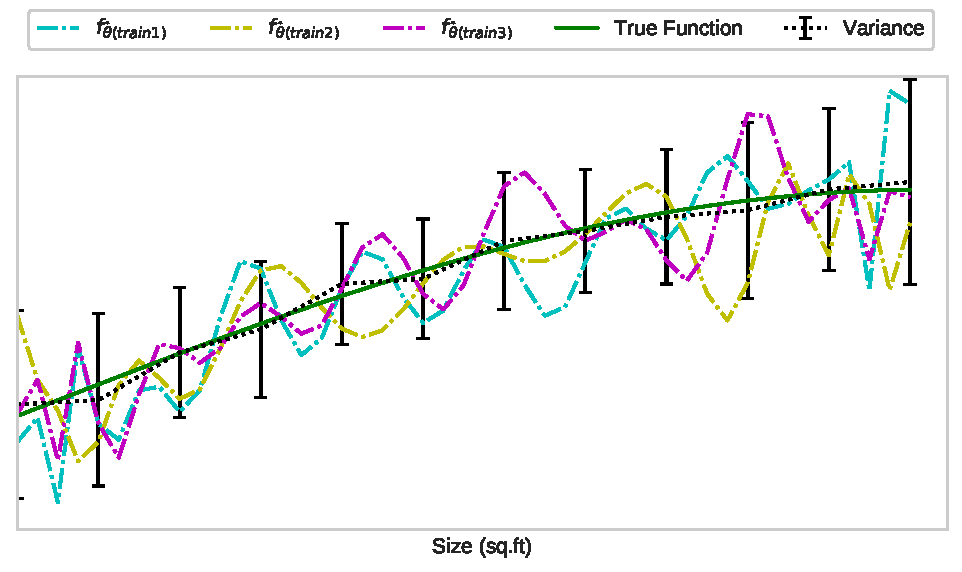
\includegraphics[width=0.8\textwidth]{../assets/bias-variance/figures/var4.pdf}}
\end{center}

\begin{alertbox}
\textbf{High Variance = Overfitting:} Model memorizes training data instead of learning general patterns
\end{alertbox}
\end{frame}

\begin{frame}{The Bias-Variance Tradeoff: The Central Tension}
\begin{center}
\fitpic{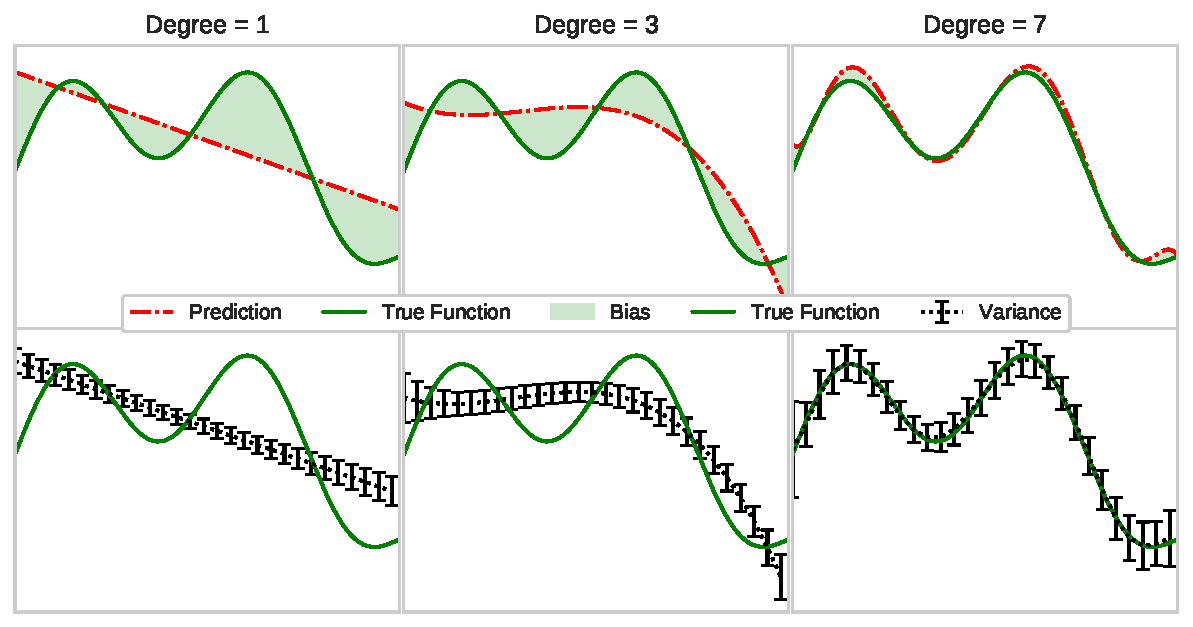
\includegraphics[width=0.95\textwidth]{../assets/bias-variance/figures/bv-2.pdf}}
\end{center}

\begin{alertbox}{The Fundamental Tradeoff}
\begin{itemize}
\item \textbf{Simple models:} High bias, low variance
\item \textbf{Complex models:} Low bias, high variance
\item \textbf{Optimal complexity:} Balance between the two
\end{itemize}
\end{alertbox}

\begin{keypointsbox}
\textbf{Key Insight:} We cannot minimize both bias and variance simultaneously!
\end{keypointsbox}
\end{frame}

\section{Mathematical Derivation: The Bias-Variance Decomposition}

\begin{frame}{Why Mathematical Analysis Matters}
\begin{definitionbox}{The Goal}
\textbf{Question:} Can we mathematically prove that error = bias$^2$ + variance + noise?
\end{definitionbox}

\begin{keypointsbox}{Why This Matters}
\begin{itemize}
\item \textbf{Theoretical foundation:} Understand the fundamental nature of learning
\item \textbf{Model selection:} Know exactly what we're trading off
\item \textbf{Algorithm design:} Create methods that explicitly balance bias and variance
\end{itemize}
\end{keypointsbox}

\begin{examplebox}{Expected Error Across All Possible Datasets}
$$E_{\mathcal{D}}[\text{Error}] = \text{Average error over all possible training sets } \mathcal{D}$$
\end{examplebox}

\begin{alertbox}
\textbf{Key Insight:} We need to average over the randomness in training set selection
\end{alertbox}
\end{frame}

\begin{frame}{Setting Up the Mathematical Framework}
\begin{definitionbox}{What We Want to Prove}
$$E[\text{Error}] = \text{Noise} + \text{Bias}^2 + \text{Variance}$$
\end{definitionbox}

\begin{keypointsbox}{Our Approach}
\begin{enumerate}
\item Start with prediction error at a single point
\item Use squared loss: $(y - \hat{f}(x))^2$
\item Take expectation over all sources of randomness
\item Apply algebraic manipulation to separate terms
\end{enumerate}
\end{keypointsbox}

\begin{examplebox}{Sources of Randomness}
\begin{itemize}
\item \textbf{Training set:} Which data points we observe
\item \textbf{Noise:} Random variation in target values
\end{itemize}
\end{examplebox}
\end{frame}

\begin{frame}{Mathematical Setup: Defining the Components}
\begin{definitionbox}{True Relationship with Noise}
$$y = f_{\text{true}}(x) + \epsilon \quad \text{where } \epsilon \sim \mathcal{N}(0, \sigma^2)$$
\end{definitionbox}

\begin{keypointsbox}{Key Definitions}
\begin{itemize}
\item $f_{\text{true}}(x)$: The unknown true function
\item $\hat{f}(x)$: Our model's prediction (depends on training data)
\item $E[\hat{f}(x)]$: Expected prediction over all possible training sets
\item $\epsilon$: Irreducible noise with variance $\sigma^2$
\end{itemize}
\end{keypointsbox}

\begin{center}
\fitpic{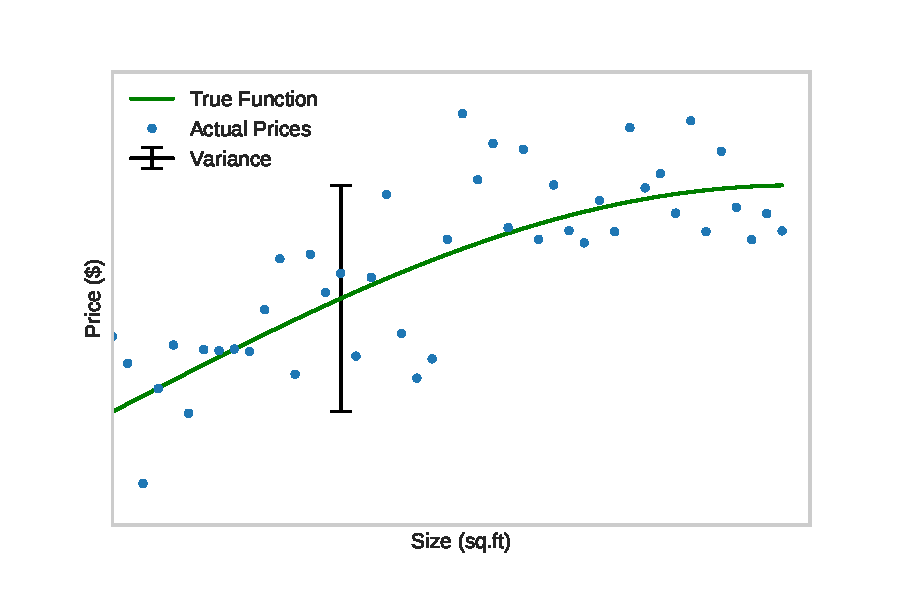
\includegraphics[width=0.6\textwidth]{../assets/bias-variance/figures/data_var.pdf}}
\end{center}
\end{frame}

\begin{frame}{Formal Definitions: Bias and Variance}
\begin{definitionbox}{Bias}
$$\text{Bias}(x) = f_{\text{true}}(x) - E[\hat{f}(x)]$$
\textbf{Systematic error:} Difference between truth and expected prediction
\end{definitionbox}

\begin{definitionbox}{Variance}
$$\text{Variance}(x) = E[(\hat{f}(x) - E[\hat{f}(x)])^2]$$
\textbf{Prediction instability:} Expected squared deviation from mean prediction
\end{definitionbox}

\begin{center}
\fitpic{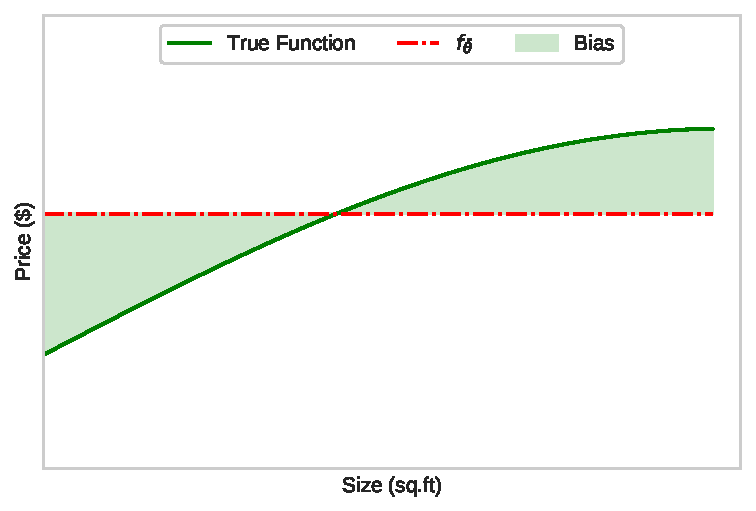
\includegraphics[width=0.6\textwidth]{../assets/bias-variance/figures/bias6.pdf}}
\end{center}

\begin{keypointsbox}
\textbf{Note:} Both bias and variance are properties of the learning algorithm, not individual models
\end{keypointsbox}
\end{frame}

\begin{frame}{The Main Theorem: Bias-Variance Decomposition}
\begin{alertbox}{The Fundamental Result}
\textbf{For any point $x$ and any learning algorithm:}
$$E[(y - \hat{f}(x))^2] = \sigma^2 + [\text{Bias}(x)]^2 + \text{Variance}(x)$$
\end{alertbox}

\begin{definitionbox}{Component Interpretation}
\begin{itemize}
\item $\sigma^2$: \textbf{Irreducible error} (noise)
\item $[\text{Bias}(x)]^2$: \textbf{Systematic error} (underfitting)
\item $\text{Variance}(x)$: \textbf{Random error} (overfitting)
\end{itemize}
\end{definitionbox}

\begin{keypointsbox}
\textbf{Coming Up:} We'll prove this step-by-step using careful algebraic manipulation
\end{keypointsbox}
\end{frame}

\begin{frame}{Starting the Proof: Expected Squared Error}
\begin{definitionbox}{What We're Proving}
$$E[(y - \hat{f}(x))^2] = \sigma^2 + [\text{Bias}(x)]^2 + \text{Variance}(x)$$
\end{definitionbox}

\begin{keypointsbox}{Our Strategy}
\begin{enumerate}
\item Start with squared error: $(y - \hat{f}(x))^2$
\item Add and subtract strategic terms
\item Expand and use linearity of expectation
\item Show cross-terms cancel out
\item Identify the three components
\end{enumerate}
\end{keypointsbox}

\begin{examplebox}{Key Insight}
\textbf{The "add and subtract" trick:} We'll add and subtract $f_{\text{true}}(x)$ and $E[\hat{f}(x)]$ to create the terms we need
\end{examplebox}
\end{frame}

\begin{frame}{Step 1: Setting Up the Expectation}
\begin{definitionbox}{Squared Loss at Point $x$}
\textbf{Individual prediction error:} $(y - \hat{f}(x))^2$
\end{definitionbox}

\begin{keypointsbox}{Taking Expectations}
\textbf{Expected error over all randomness:}
$$E_{\mathcal{D}, y}[(y - \hat{f}(x))^2]$$
where:
\begin{itemize}
\item $\mathcal{D}$: Random training set
\item $y$: Random target (includes noise)
\end{itemize}
\end{keypointsbox}

\begin{examplebox}{Why Two Sources of Randomness?}
\begin{itemize}
\item \textbf{Training set randomness:} Which data points we see affects $\hat{f}$
\item \textbf{Target randomness:} Noise affects the true $y$ value
\end{itemize}
\end{examplebox}
\end{frame}

\begin{frame}{Step 2: The Add-and-Subtract Trick}
\begin{keypointsbox}{Starting Point}
$$E[(y - \hat{f}(x))^2]$$
\end{keypointsbox}

\begin{examplebox}{Strategic Addition and Subtraction}
\textbf{Add and subtract } $f_{\text{true}}(x)$:
$$E[(y - f_{\text{true}}(x) + f_{\text{true}}(x) - \hat{f}(x))^2]$$
\end{examplebox}

\begin{definitionbox}{Grouping Terms}
$$E[\underbrace{(y - f_{\text{true}}(x))}_{\text{noise: } \epsilon} + \underbrace{(f_{\text{true}}(x) - \hat{f}(x))}_{\text{prediction error}}]^2$$
\end{definitionbox}

\begin{alertbox}
\textbf{Key Insight:} We've separated the noise from the prediction error!
\end{alertbox}
\end{frame}

\begin{frame}{Step 3A: Expanding the Square}
\begin{keypointsbox}{Starting with Our Expression}
$$E[\underbrace{(y - f_{\text{true}}(x))}_{\epsilon} + \underbrace{(f_{\text{true}}(x) - \hat{f}(x))}_{\text{prediction error}}]^2$$
\end{keypointsbox}

\begin{examplebox}{Apply $(a + b)^2 = a^2 + 2ab + b^2$}
\textbf{Let:} $a = \epsilon$ and $b = (f_{\text{true}}(x) - \hat{f}(x))$

\textbf{Then:} $(a + b)^2 = a^2 + 2ab + b^2$
\end{examplebox}
\end{frame}

\begin{frame}{Step 3B: The Expanded Form}
\begin{definitionbox}{After Expansion}
$$E[\epsilon^2 + 2\epsilon(f_{\text{true}}(x) - \hat{f}(x)) + (f_{\text{true}}(x) - \hat{f}(x))^2]$$
\end{definitionbox}

\begin{keypointsbox}{Apply Linearity of Expectation}
$$E[\epsilon^2] + 2E[\epsilon(f_{\text{true}}(x) - \hat{f}(x))] + E[(f_{\text{true}}(x) - \hat{f}(x))^2]$$
\end{keypointsbox}
\end{frame}

\begin{frame}{Step 3C: Naming the Three Terms}
\begin{definitionbox}{Our Three Terms}
\begin{itemize}
\item \textbf{Term 1:} $E[\epsilon^2]$ (the noise term)
\item \textbf{Term 2:} $2E[\epsilon(f_{\text{true}}(x) - \hat{f}(x))]$ (cross-term)
\item \textbf{Term 3:} $E[(f_{\text{true}}(x) - \hat{f}(x))^2]$ (prediction error)
\end{itemize}
\end{definitionbox}

\begin{keypointsbox}{Our Strategy}
\textbf{We'll analyze each term separately:}
\begin{itemize}
\item Term 1 → Noise ($\sigma^2$)
\item Term 2 → Will be zero! 
\item Term 3 → Bias$^2$ + Variance
\end{itemize}
\end{keypointsbox}
\end{frame}

\begin{frame}{Step 4A: Analyzing Term 1 - Setup}
\begin{definitionbox}{Term 1 Recall}
$$\text{Term 1} = E[\epsilon^2]$$
where $\epsilon = y - f_{\text{true}}(x)$ is the noise
\end{definitionbox}

\begin{keypointsbox}{Key Insight}
\textbf{Independence:} The noise $\epsilon$ doesn't depend on our training set!
\begin{itemize}
\item Noise is a property of the data generation process
\item Training set selection doesn't affect noise level
\item Noise is the same regardless of which model we choose
\end{itemize}
\end{keypointsbox}
\end{frame}

\begin{frame}{Step 4B: Term 1 - The Calculation}
\begin{examplebox}{By Definition of Noise}
$$\epsilon = y - f_{\text{true}}(x) \sim \mathcal{N}(0, \sigma^2)$$
\end{examplebox}

\begin{keypointsbox}{Therefore}
$$E[\epsilon^2] = \text{Var}(\epsilon) + (E[\epsilon])^2 = \sigma^2 + 0^2 = \sigma^2$$
\end{keypointsbox}

\begin{alertbox}{Result}
$$\boxed{\text{Term 1} = \sigma^2}$$
\textbf{This is our irreducible error (noise)!}
\end{alertbox}
\end{frame}

\begin{frame}{Step 5A: Analyzing Term 2 - Setup}
\begin{definitionbox}{Term 2 Recall}
$$\text{Term 2} = 2E[\epsilon(f_{\text{true}}(x) - \hat{f}(x))]$$
\end{definitionbox}

\begin{keypointsbox}{Key Independence Property}
\textbf{Crucial insight:} $\epsilon$ (noise) is independent of $\hat{f}(x)$ (our prediction)
\begin{itemize}
\item Noise occurs in nature, regardless of our model
\item Our model $\hat{f}$ depends only on training data
\item Training data and future noise are independent
\end{itemize}
\end{keypointsbox}
\end{frame}

\begin{frame}{Step 5B: Term 2 - Why Independence Matters}
\begin{examplebox}{What Independence Means}
\textbf{If $X$ and $Y$ are independent:} $E[XY] = E[X] \cdot E[Y]$

\textbf{In our case:}
\begin{itemize}
\item $X = \epsilon$ (noise)
\item $Y = f_{\text{true}}(x) - \hat{f}(x)$ (prediction error)
\end{itemize}
\end{examplebox}

\begin{keypointsbox}{Apply Independence}
$$E[\epsilon(f_{\text{true}}(x) - \hat{f}(x))] = E[\epsilon] \cdot E[f_{\text{true}}(x) - \hat{f}(x)]$$
\end{keypointsbox}
\end{frame}

\begin{frame}{Step 5C: Term 2 - The Final Calculation}
\begin{examplebox}{Using $E[\epsilon] = 0$}
$$E[\epsilon(f_{\text{true}}(x) - \hat{f}(x))] = E[\epsilon] \cdot E[f_{\text{true}}(x) - \hat{f}(x)]$$
$$= 0 \cdot E[f_{\text{true}}(x) - \hat{f}(x)] = 0$$
\end{examplebox}

\begin{alertbox}{Result}
$$\boxed{\text{Term 2} = 2 \times 0 = 0}$$
\textbf{The cross-term vanishes completely!}
\end{alertbox}

\begin{keypointsbox}{Why This Matters}
Cross-terms often make math messy, but here they cancel out beautifully!
\end{keypointsbox}
\end{frame}

\begin{frame}{Step 6: Analyzing Term 3 - The Prediction Error}
\begin{definitionbox}{Term 3 Analysis}
$$E[(f_{\text{true}}(x) - \hat{f}(x))^2]$$
\end{definitionbox}

\begin{keypointsbox}{Another Independence}
\textbf{Key insight:} $(f_{\text{true}}(x) - \hat{f}(x))$ doesn't depend on the noise $\epsilon$
\begin{itemize}
\item $f_{\text{true}}(x)$ is deterministic
\item $\hat{f}(x)$ depends only on training inputs/outputs (not future noise)
\end{itemize}
\end{keypointsbox}

\begin{examplebox}{Simplification}
$$E[(f_{\text{true}}(x) - \hat{f}(x))^2] = \text{MSE of prediction}$$
\end{examplebox}

\begin{alertbox}{Coming Up}
\textbf{This MSE term is where bias and variance hide!} We need to decompose it further...
\end{alertbox}
\end{frame}

\begin{frame}{Interim Summary: Progress So Far}
\begin{definitionbox}{What We Have}
$$E[(y - \hat{f}(x))^2] = \sigma^2 + 0 + E[(f_{\text{true}}(x) - \hat{f}(x))^2]$$
$$= \sigma^2 + E[(f_{\text{true}}(x) - \hat{f}(x))^2]$$
\end{definitionbox}

\begin{keypointsbox}{Next Challenge}
\textbf{Goal:} Decompose $E[(f_{\text{true}}(x) - \hat{f}(x))^2]$ into bias$^2$ + variance
\end{keypointsbox}

\begin{examplebox}{Strategy for Next Step}
\textbf{Another add-and-subtract trick:} We'll add and subtract $E[\hat{f}(x)]$ inside the MSE term
\end{examplebox}
\end{frame}

\begin{frame}{Step 7A: The Second Decomposition - Setup}
\begin{keypointsbox}{Current Status}
$$E[(y - \hat{f}(x))^2] = \sigma^2 + E[(f_{\text{true}}(x) - \hat{f}(x))^2]$$
\end{keypointsbox}

\begin{examplebox}{Our Next Challenge}
\textbf{Goal:} Break down $E[(f_{\text{true}}(x) - \hat{f}(x))^2]$ into bias$^2$ + variance
\end{examplebox}

\begin{keypointsbox}{Strategy}
\textbf{Another add-and-subtract trick!} We'll use $E[\hat{f}(x)]$ (the expected prediction)
\end{keypointsbox}
\end{frame}

\begin{frame}{Step 7B: The Second Add-and-Subtract Trick}
\begin{definitionbox}{Starting Point}
$$E[(f_{\text{true}}(x) - \hat{f}(x))^2]$$
\end{definitionbox}

\begin{examplebox}{Add and Subtract $E[\hat{f}(x)]$}
$$E[(f_{\text{true}}(x) - E[\hat{f}(x)] + E[\hat{f}(x)] - \hat{f}(x))^2]$$
\end{examplebox}

\begin{keypointsbox}{Grouping the Terms}
$$E[\underbrace{(f_{\text{true}}(x) - E[\hat{f}(x)])}_{\text{bias}} + \underbrace{(E[\hat{f}(x)] - \hat{f}(x))}_{\text{variance deviation}}]^2$$
\end{keypointsbox}

\begin{alertbox}
\textbf{Perfect!} We've separated bias and variance components
\end{alertbox}
\end{frame}

\begin{frame}{Step 8A: Setting Up the Final Expansion}
\begin{keypointsbox}{Our Current Expression}
$$E[(\text{bias} + \text{variance deviation})^2]$$
\end{keypointsbox}

\begin{definitionbox}{Let's Define Clearly}
\begin{itemize}
\item $\alpha = f_{\text{true}}(x) - E[\hat{f}(x)]$ (the bias)
\item $\beta = E[\hat{f}(x)] - \hat{f}(x)$ (deviation from expected prediction)
\end{itemize}
\end{definitionbox}

\begin{keypointsbox}{What We're About to Do}
Expand $(\alpha + \beta)^2$ and analyze each term separately
\end{keypointsbox}
\end{frame}

\begin{frame}{Step 8B: Expanding the Square}
\begin{examplebox}{Using $(a + b)^2 = a^2 + 2ab + b^2$}
$$E[(\alpha + \beta)^2] = E[\alpha^2 + 2\alpha\beta + \beta^2]$$
\end{examplebox}

\begin{keypointsbox}{Apply Linearity of Expectation}
$$E[\alpha^2] + 2E[\alpha\beta] + E[\beta^2]$$
\end{keypointsbox}

\begin{definitionbox}{Three Terms to Analyze}
\begin{itemize}
\item \textbf{Term A:} $E[\alpha^2]$ 
\item \textbf{Term B:} $2E[\alpha\beta]$ 
\item \textbf{Term C:} $E[\beta^2]$ 
\end{itemize}
\end{definitionbox}
\end{frame}

\begin{frame}{Step 9A: Analyzing Term A - The Bias Term}
\begin{definitionbox}{Term A Recall}
$$E[\alpha^2] = E[(f_{\text{true}}(x) - E[\hat{f}(x)])^2]$$
where $\alpha = f_{\text{true}}(x) - E[\hat{f}(x)]$
\end{definitionbox}

\begin{keypointsbox}{Critical Insight}
\textbf{$\alpha$ is deterministic (not random)!}
\begin{itemize}
\item $f_{\text{true}}(x)$ is a fixed function value
\item $E[\hat{f}(x)]$ is the expected prediction (a constant)
\end{itemize}
\end{keypointsbox}
\end{frame}

\begin{frame}{Step 9B: Why Deterministic Matters}
\begin{examplebox}{When Something is Deterministic}
\textbf{If $c$ is a constant:} $E[c] = c$

\textbf{In our case:} $\alpha = f_{\text{true}}(x) - E[\hat{f}(x)]$ is constant
\end{examplebox}

\begin{keypointsbox}{Therefore}
$$E[\alpha^2] = E[(f_{\text{true}}(x) - E[\hat{f}(x)])^2] = (f_{\text{true}}(x) - E[\hat{f}(x)])^2$$
\end{keypointsbox}

\begin{alertbox}{Result}
$$\boxed{E[\alpha^2] = [\text{Bias}(x)]^2}$$
\textbf{First component: Bias squared!}
\end{alertbox}
\end{frame}

\begin{frame}{Step 10A: Analyzing Term B - The Cross-Term}
\begin{definitionbox}{Term B Recall}
$$E[\alpha\beta] = E[(f_{\text{true}}(x) - E[\hat{f}(x)])(E[\hat{f}(x)] - \hat{f}(x))]$$
\end{definitionbox}

\begin{keypointsbox}{Key Insight}
\textbf{$\alpha$ is deterministic:} $(f_{\text{true}}(x) - E[\hat{f}(x)])$ is a constant
\begin{itemize}
\item Can factor constants out of expectations
\item $E[c \cdot X] = c \cdot E[X]$ when $c$ is constant
\end{itemize}
\end{keypointsbox}
\end{frame}

\begin{frame}{Step 10B: Factoring Out the Constant}
\begin{examplebox}{Using the Constant Rule}
$$E[\alpha\beta] = E[(f_{\text{true}}(x) - E[\hat{f}(x)])(E[\hat{f}(x)] - \hat{f}(x))]$$
$$= (f_{\text{true}}(x) - E[\hat{f}(x)]) \cdot E[E[\hat{f}(x)] - \hat{f}(x)]$$
\end{examplebox}

\begin{keypointsbox}{Simplifying the Expectation}
$$E[E[\hat{f}(x)] - \hat{f}(x)] = E[\hat{f}(x)] - E[\hat{f}(x)] = 0$$
\end{keypointsbox}

\begin{alertbox}{Result}
$$\boxed{E[\alpha\beta] = \text{bias} \times 0 = 0}$$
\textbf{Cross-term vanishes again!}
\end{alertbox}
\end{frame}

\begin{frame}{Step 11A: Analyzing Term C - The Variance Term}
\begin{definitionbox}{Term C Recall}
$$E[\beta^2] = E[(E[\hat{f}(x)] - \hat{f}(x))^2]$$
where $\beta = E[\hat{f}(x)] - \hat{f}(x)$
\end{definitionbox}

\begin{keypointsbox}{Does This Look Familiar?}
\textbf{Compare with the definition of variance:}
$$\text{Variance}(X) = E[(X - E[X])^2]$$
\end{keypointsbox}
\end{frame}

\begin{frame}{Step 11B: Recognizing the Variance Formula}
\begin{examplebox}{Rewriting Term C}
$$E[\beta^2] = E[(E[\hat{f}(x)] - \hat{f}(x))^2]$$
$$= E[(\hat{f}(x) - E[\hat{f}(x)])^2]$$
\end{examplebox}

\begin{keypointsbox}{This is Exactly...}
$$\text{Variance}(\hat{f}(x)) = E[(\hat{f}(x) - E[\hat{f}(x)])^2]$$
\end{keypointsbox}

\begin{alertbox}{Result}
$$\boxed{E[\beta^2] = \text{Variance}(\hat{f}(x))}$$
\textbf{Final component: Variance!}
\end{alertbox}
\end{frame}

\begin{frame}{The Complete Bias-Variance Decomposition}
\begin{alertbox}{Putting It All Together}
$$E[(y - \hat{f}(x))^2] = \sigma^2 + [\text{Bias}(x)]^2 + \text{Variance}(x)$$
\end{alertbox}

\begin{definitionbox}{Component Summary}
\begin{itemize}
\item $\sigma^2$ = \textbf{Irreducible error} (noise in data)
\item $[\text{Bias}(x)]^2$ = \textbf{Systematic error} (model assumptions)
\item $\text{Variance}(x)$ = \textbf{Random error} (training set sensitivity)
\end{itemize}
\end{definitionbox}

\begin{keypointsbox}{The Fundamental Tradeoff}
\begin{itemize}
\item \textbf{Reduce bias:} Use more complex models → Increase variance
\item \textbf{Reduce variance:} Use simpler models → Increase bias
\item \textbf{Optimal complexity:} Minimize bias$^2$ + variance
\end{itemize}
\end{keypointsbox}

\begin{examplebox}{Practical Implications}
\textbf{This decomposition explains:}
\begin{itemize}
\item Why cross-validation works
\item How to choose model complexity
\item The mathematics behind regularization
\end{itemize}
\end{examplebox}
\end{frame}

\begin{frame}{Summary: The Bias-Variance Tradeoff}
\begin{definitionbox}{What We've Proven}
\textbf{Every prediction error can be decomposed as:}
$$\text{Total Error} = \text{Noise} + \text{Bias}^2 + \text{Variance}$$
\end{definitionbox}

\begin{keypointsbox}{Key Takeaways}
\begin{itemize}
\item \textbf{Noise:} Cannot be reduced (irreducible)
\item \textbf{Bias:} Reduced by increasing model complexity
\item \textbf{Variance:} Reduced by decreasing model complexity
\item \textbf{Optimal model:} Balances bias and variance
\end{itemize}
\end{keypointsbox}

\begin{alertbox}{Practical Applications}
\begin{itemize}
\item \textbf{Model selection:} Choose complexity to minimize total error
\item \textbf{Ensemble methods:} Reduce variance while maintaining low bias
\item \textbf{Regularization:} Explicitly control the bias-variance tradeoff
\item \textbf{Cross-validation:} Estimate the full error decomposition
\end{itemize}
\end{alertbox}
\end{frame}

\end{document}